% Extracted from LaTeX-examples-master/tikz/triangle-9-point-circle.
% tkzDefCircle returns the circumcenter and first circumference point.
\documentclass[border=3pt]{standalone}
\usepackage{tikz}
\usepackage{tkz-euclide}

\begin{document}
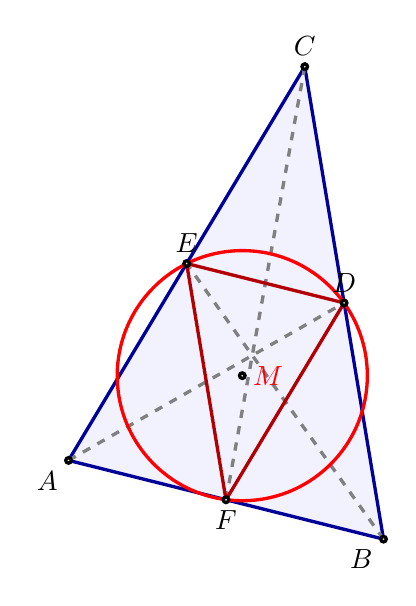
\begin{tikzpicture}[very thick]
  \tkzDefPoint(0,1){A}
  \tkzDefPoint(4,0){B}
  \tkzDefPoint(3,6){C}
  \tkzDefMidPoint(A,B)\tkzGetPoint{F}
  \tkzDefMidPoint(A,C)\tkzGetPoint{E}
  \tkzDefMidPoint(B,C)\tkzGetPoint{D}
  \tkzDefCircle[circum,/tikz/overlay](D,E,F)\tkzGetPoints{M}{P}\tkzGetLength{rNine}

  \fill[blue!5] (A) -- (B) -- (C) -- cycle;
  \draw[blue!60!black] (A) -- (B) -- (C) -- cycle;
  \draw[dashed,gray] (A) -- (D) (B) -- (E) (C) -- (F);
  \draw[red!70!black] (D) -- (E) -- (F) -- cycle;
  \tkzDrawCircle[color=red,very thick](M,P)

  \tkzDrawPoints(A,B,C,D,E,F,M)
  \tkzLabelPoints[below left](A,B)
  \tkzLabelPoints[above](C,D,E)
  \tkzLabelPoints[below](F)
  \tkzLabelPoints[right,red](M)
\end{tikzpicture}
\end{document}
